% !TEX root = ../thesis-example.tex
%
%************************************************
% Kern der Arbeit
%************************************************
\chapter{Reranking mittels CTR}
\label{sec:Reranking}

Aufgrund der Diskussionen zu den Problemstellungen des Lösungsansatzes im vorhergehenden Kapitel \ref{sec:Grundlagen}, kennen wir verschiedene Varianten der Lösungsansätze und deren Eigenschaften. In diesem Kapitel geht es nun darum, aus diesem Wissen unseren detaillierten Lösungsansatz des Reranking-Algorithmus zusammenzubauen. Dazu werden wir uns zuerst den Prozess des neuen Reranking-Algorithmus anschauen. Wie wir zu diesem Prozessbild kommen, lernen wir anschließend in der Methodik kennen. Diese baut auf der Methodik aus Kapitel \ref{sec:Einfuehrung:Methodik} auf. Dabei werden wir ausführlich die Beweggründe zum gewählten Lösungsansatz kennenlernen und die theoretische Umsetzung diskutieren. Im nächsten Kapitel folgt dann die praktische Umsetzung des hier ausgearbeiteten Lösungsansatzes.

%Prozessaufbau des Lösungsansatzes
%----------------------------------------------------------------

\section{Prozessaufbau des Lösungsansatzes}
\label{sec:Reranking:Prozessaufbau}

\subsection{Prozessaufbau als Bild}
\label{sec:Reranking:Prozessaufbau:ProzessaufbauBild}

\begin{figure}[H]
\centering
\vspace{-1em}
\caption[Prozessaufbau des Lösungsansatzes]{Prozessaufbau des Lösungsansatzes}
\label{fig:Prozessaufbau}
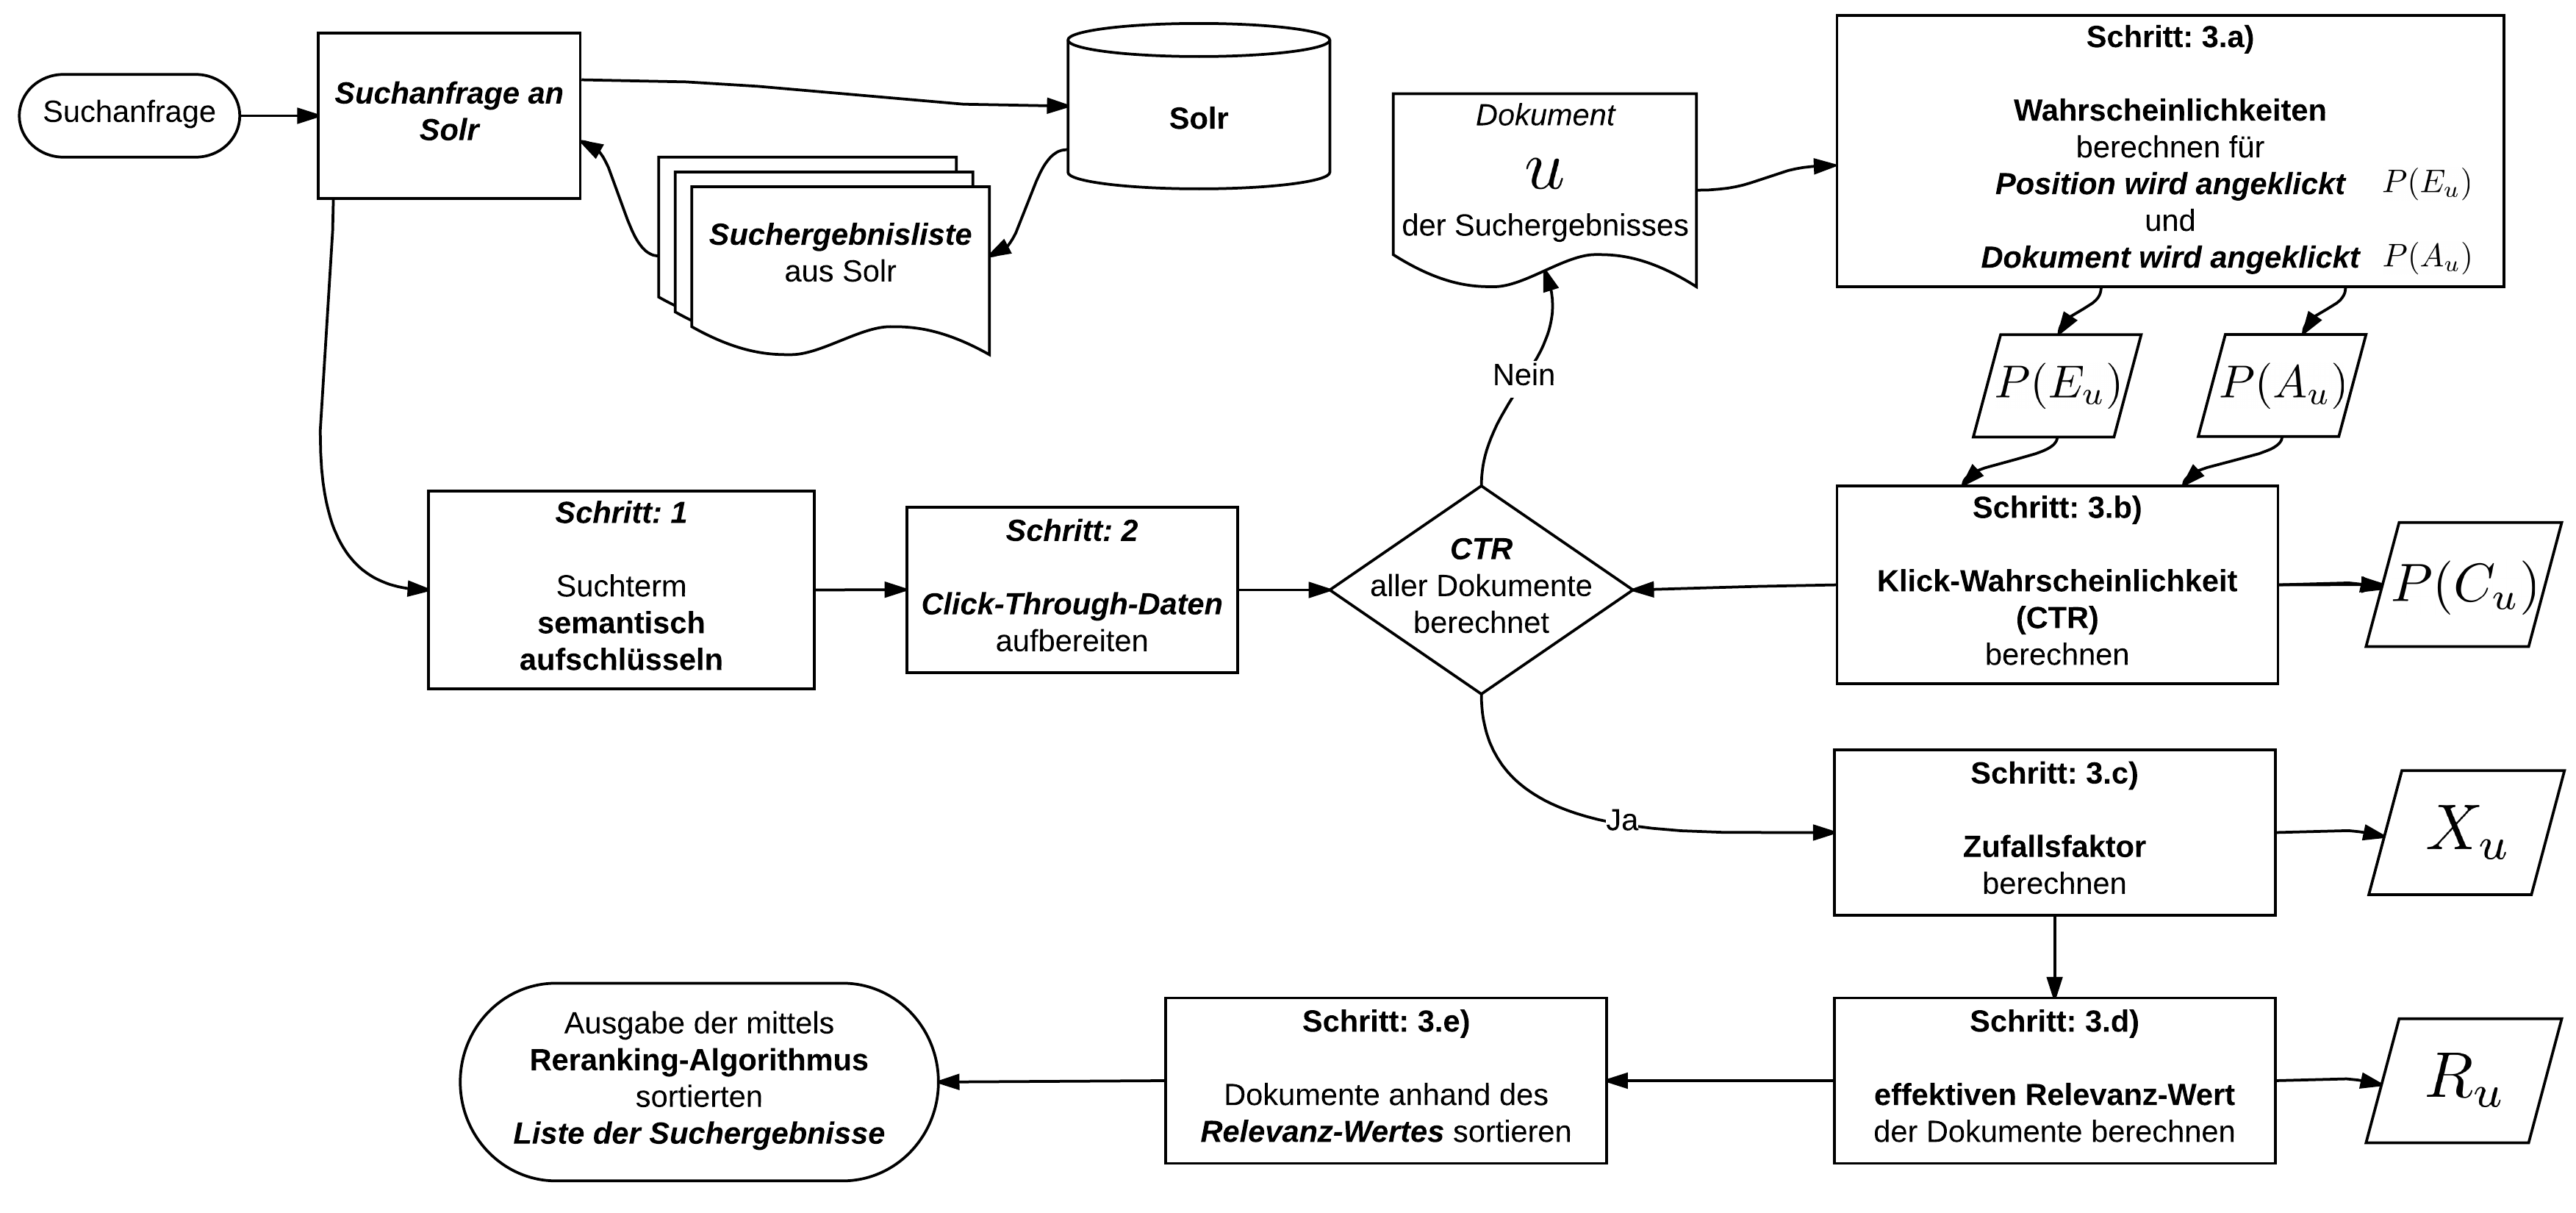
\includegraphics[width=\linewidth]{gfx/ProzessaufbauBild}
\vspace{-2em}
\end{figure}
		
%Methodik
%----------------------------------------------------------------

\section{Methodik}
\label{sec:Reranking:Methodik}

Wie bereits in der Einführung zu diesem Kapitel besprochen, haben wir gelernt wie Click-Through-Daten entstehen, wie sie zu lesen sind und wie wir Aussagen zu ihnen treffen können. Nun werden wir mithilfe dieses Wissens, die CTR der Dokumente berechnen. Mithilfe der berechneten Click-Through-Daten werden wir dann ein \textit{Reranking} der Suchresultate durchführen, bevor diese dem User präsentiert werden. So wollen wir die Userrelevanz mittels CTR in die Suche einbinden. Die Vorgehensweise dazu sieht wie folgt aus.

\subsection{Suchterm Segmentierung}
\label{sec:Reranking:Methodik:SuchtermSegmentierung}

Um alle relevanten Click-Through-Daten lesen zu können, müssen wir zunächst den Suchterm auftrennen, wie in Kapitel \ref{sec:Grundlagen:Grundbegriffe:SemantikUserInteraktionen:ProblemstellungenClick-Through-Daten} angesprochen. Der Prozess dazu sieht wie folgt aus:

\begin{figure}[H]
\centering
\vspace{-1em}
\caption[Prozess der semantischen Segmentierung des Suchterms]{Prozess der semantischen Segmentierung des Suchterms}
\label{fig:SemantischeSegmentierung}
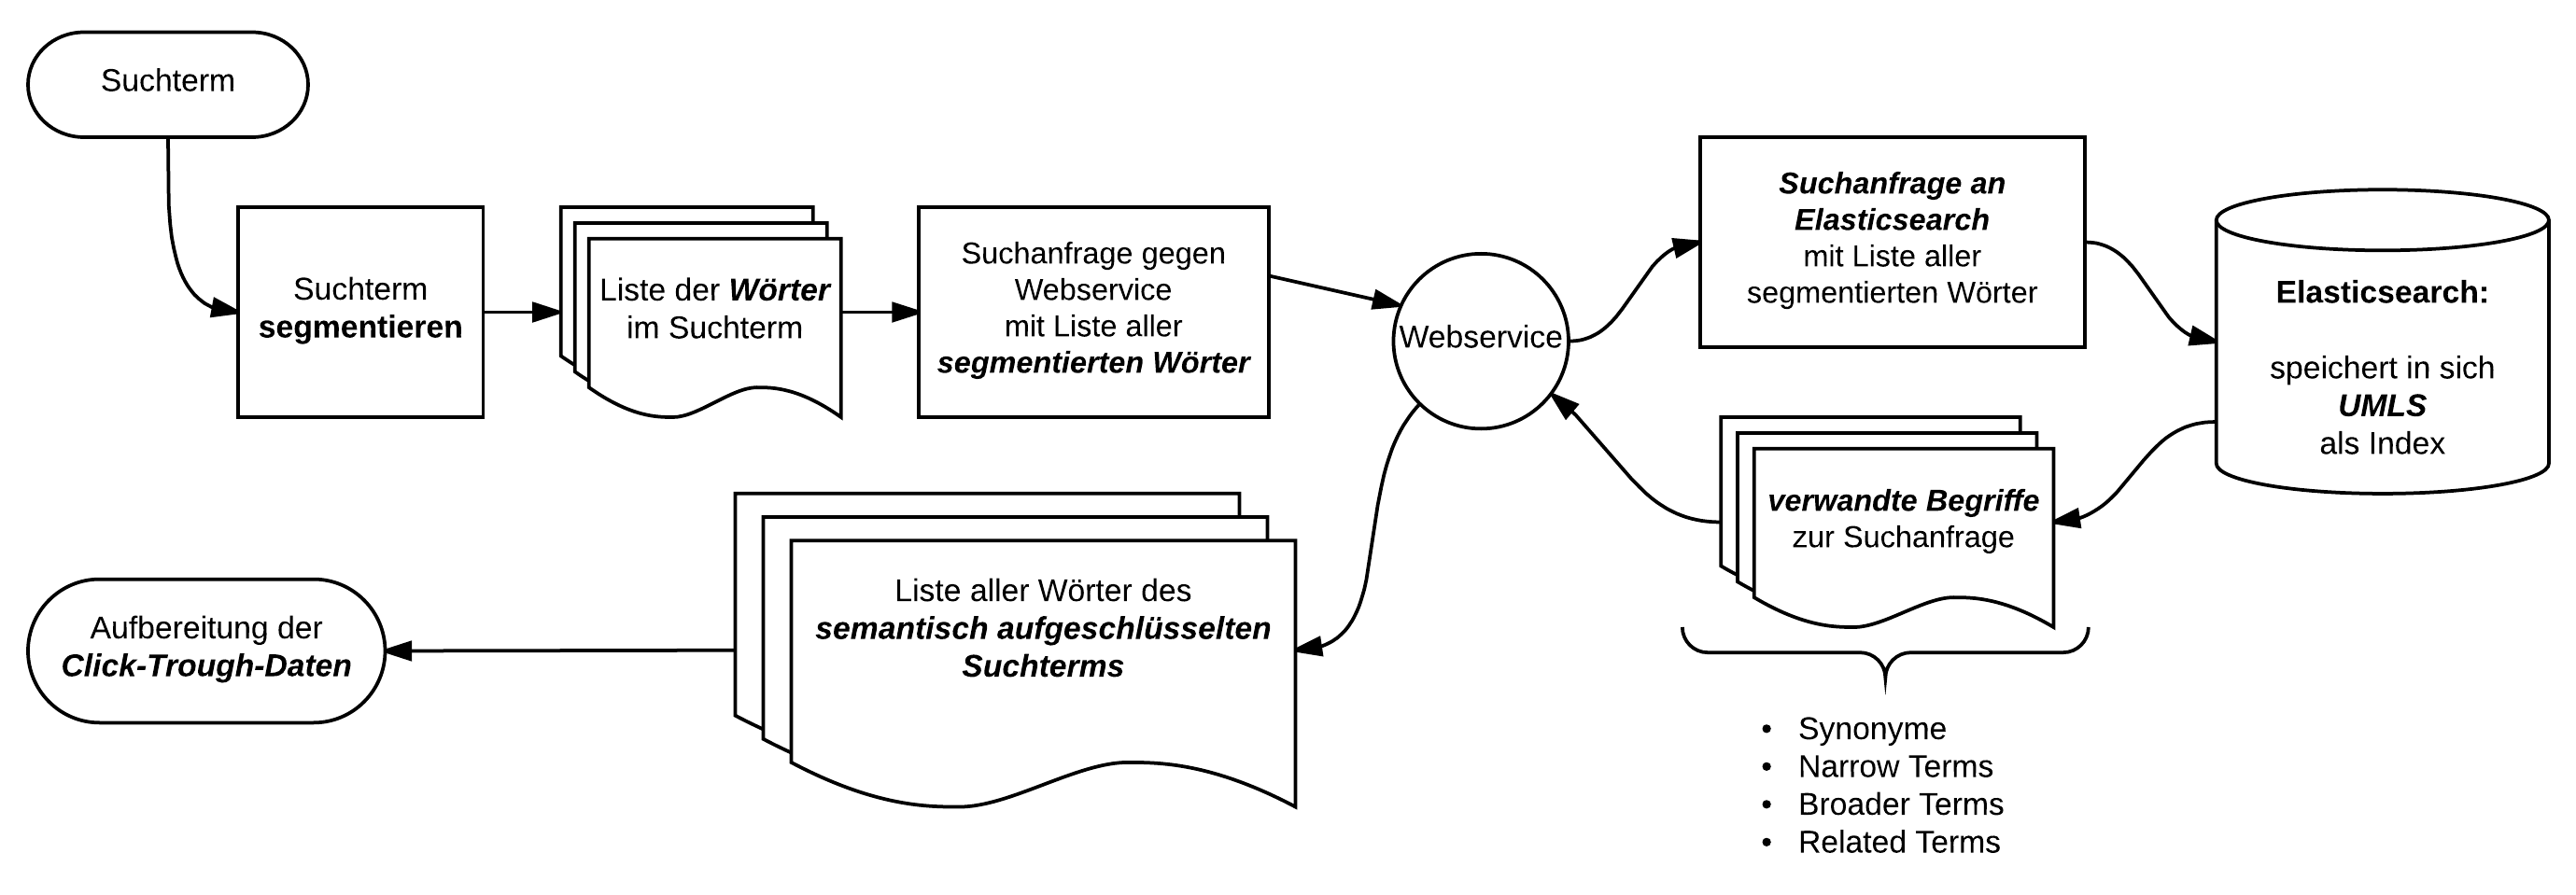
\includegraphics[width=\linewidth]{gfx/SuchtermSegmentierung}
\vspace{-2em}
\end{figure} 

\subsubsection{Suchterm semantisch aufschlüsseln mittels Segmentierung}
\label{sec:Reranking:Methodik:SuchtermSegmentierung:SuchtermSegmentierung}

Die Auftrennung des Suchterms in die einzelne Worte können wir mithilfe einer Segmentierung\footnote{Bezeichnet die Aufteilung in Abschnitte, in diesem Fall in einzelne Worte} durchführen. Hier könnten wir uns überlegen, zusätzlich mit Stoppwörtern\footnote{Stoppwörter sind Wörter, die sehr häufig auftreten und für gewöhnlich keine Relevanz für den Dokumentinhalt besitzen}, nicht relevante Wörter aus dem Suchterm zu entfernen. Dieses Verfahren macht aber im Springermedizin-Kontext keinen Sinn. Wie in Kapitel \ref{sec:Einfuehrung:Problemstellung:Userrelevanz} angesprochen, suchen die User der Springermedizin-Applikation oft mit einschlägig, fundierten Fachbegriffen. Wir gehen darum davon aus, dass alle Wörter des verwendeten Suchterms für das Suchergebnis relevant sind. Diese Erkenntnis basiert auf Aussagen der Redakteure von Springermedizin und Webtrekk-Analysen der meist gesuchtesten Suchtermen der letzten Monate. Auch sind Stoppwörter veraltet und werden in modernen Information Retrieval Verfahren nicht mehr eingesetzt. Wir verzichten darum auf den Einstatz von Stoppwörtern.

\subsubsection{Suchterm semantisch erweitern mittels Thesaurus}
\label{sec:Reranking:Methodik:SuchtermSegmentierung:SuchtermThesaurus}

Wie ebenfalls in Kapitel \ref{sec:Grundlagen:Grundbegriffe:SemantikUserInteraktionen:ProblemstellungenClick-Through-Daten} thematisiert, wollen wir die Click-Through-Daten zu unserem Suchterm um Click-Through-Daten zu verwandten Begriffen erweitern. Für diese semantische Erweiterung eines Suchwortes werden wir einen Thesaurus verwenden. Die Erweiterung umfasst zum Suchterm gleichbedeutende Begriffe (\textit{Synonyme}), sehr ähnliche Begriffe (\textit{Narrow Terms}), ähnliche Begriffe im weiteren Sinne (\textit{Broader Terms}) und verwandte Begriffe (\textit{Related Terms}). 

\paragraph{Mittels Webservice einen UMLS-Thesaurus nach relevanten Begriffen durchsuchen}
Springer Nature besitzt einen Webservice mit welchem auf den Thesaurus \textit{Unified Medical Language System}~(UMLS, siehe \cite{UMLS}) zugegriffen werden kann. Der Webservice nimmt einzelne Wörter und Wörter-Listen entgegen. Zu jedem dieser Wörter durchsucht der Webservice den Thesaurus nach den oben erwähnten Arten von verwandten Begriffen. Der Webservice verwendet für diese Suche eine Elasticsearch\footnote{Eine Elasticsearch ist eine Volltextsuchmaschine}~(siehe \cite{elasticsearch}). Die dabei gefundenen Begriffe, liefert der Webservice als Antwort zurück. Um alle relevanten Click-Through-Daten zu finden, werden wir mit dem segmentierten Suchterm eine Anfrage gegen diesen Webservice stellen und anschließend den segmentierten Suchterm um die gefundenen Begriffe erweitern. Mithilfe des erweiterten Suchterms können wir dann anschließend eine Analyse in Webtrekk starten und alle relevanten Click-Through-Daten lesen. 

\subsection{Aufbereitung Click-Through-Daten}
\label{sec:Reranking:Methodik:Click-Through-Daten}

\subsubsection{Jeder Klick auf ein Dokument ist relevant}
\label{sec:Reranking:Methodik:Click-Through-Daten:Click-Through-DatenAuswertungen}

Wie in Kapitel \ref{sec:Grundlagen:Grundbegriffe:Click-Through-Daten:UserverhaltensFeedback} beschrieben, reichen Webtrekk-Analysen für komplexe Auswertungen der Click-Through-Daten nicht aus. Wir können darum in dieser Arbeit \textit{Feedback-Strategien} für die CTR Auswertung, wie in \cite{Joachims} beschrieben, nicht verwenden. Stattdessen greifen wir wie ebenfalls in Kapitel \ref{sec:Grundlagen:Grundbegriffe:Click-Through-Daten:UserverhaltensFeedback} beschrieben auf die Click-Through Features zu, die uns Webtrekk zur Verfügung stellt. Daraus entsteht das folgende, interpretierbare Feature-Set:

\begin{table}[H]
\vspace{-.75em}
 \caption[Interpretierbares Feature-Set aus den Webtrekk Click-Through-Daten]{Interpretierbares Feature-Set aus den Webtrekk Click-Through-Daten}
\label{tab:Feature-Set}
\vspace{-.5em}
\footnotesize
\renewcommand*{\arraystretch}{1.2}
\resizebox{\textwidth}{!}{%
\begin{tabular}{ll}
\hline
\multicolumn{2}{l}{\textit{\textbf{Click-Through Features}}}                                                                      \\ \hline
\textbf{Feature}          & \textbf{Beschreibung}                                                                                 \\ \hline
\textit{Position}         & Position dieses Dokumentes im Suchergebnis (angeklickte Position)                                     \\
\textit{ClickFrequency}   & Anzahl Klicks für dieses Dokument zum angefragten Suchterm (Klick-Häufigkeit)                         \\
\textit{ClickProbability} & Klick-Wahrscheinlichkeit zum Suchterm (\textit{ClickFrequency} geteilt durch \textit{Gesamtanzahl der Klicks zum angefragten Suchterm}) \\ \hline
\end{tabular}
}
\vspace{-2em}
\end{table}

Wie wir sehen, ist unser Feature-Set im Vergleich zu dem in \cite{IWUSBI} beschriebenen, sehr stark eingeschränkt und enthält keine Relevanz-Informationen um ein Relevanz-Feedback zu den Klick-Häufigkeiten daraus ableiten zu können. Wir müssen wir darum davon ausgehen, dass jeder Klick auf ein Dokument relevant ist.

\subsubsection{Gewichtung der Click-Through-Daten}
\label{sec:Reranking:Methodik:Click-Through-Daten:Gewichtung}

Durch die semantische Aufschlüsselung des Suchterms haben wir verschieden starke Relationen zwischen Click-Through-Daten und dem Suchterm. Die Gewichtung der Stärke dieser Relation ist aber nicht Kern dieser Arbeit. Wir gehen darum davon aus, dass unabhängig der stärke der Relation zum Suchterm, alle Click-Through-Daten eine gleiche Relevanz besitzen.

\subsubsection{Berechnung der CTR}
\label{sec:Reranking:Methodik:Click-Through-Daten:Gewichtung}

\paragraph{Einfache CTR ignoriert viele Problemstellungen der Interaktion zwischen dem User und der Suche} 
Wie wir bereits wissen, stellt die CTR die Anzahl der Klicks auf ein Dokument im Verhältnis zu den gesamten Impressionen dar. Bezogen auf das in Kapitel \ref{sec:Grundlagen:Grundbegriffe:Click-Through-Daten:UserverhaltensFeedback} angesprochene Feature-Set, würden wir die \textit{ClickProbability} direkt als CTR verwenden. Dazu müssten wir nur die Click-Through-Daten eines Dokuments ins Verhältnis zu allen Click-Through-Daten für einer Suchanfrage stellen. Wie wir aber bereits in Kapitel \ref{sec:Grundlagen:Grundbegriffe:SemantikUserInteraktionen:ProblemstellungenClick-Through-Daten} gelernt haben, würden wir damit viele Problemstellungen der Interaktion des Users mit der Suche ignorieren. Deswegen haben wir uns für eine Lösung basierend auf einem Klick-Modell entschieden. 

\paragraph{Klick-Wahrscheinlichkeit als CTR für Reranking verwenden} 
Klick-Modelle versuchen die Click-Through-Daten zu interpretieren und aus ihnen ein Relevanz-Feedback zu schlussfolgern. Das machen sie mithilfe des bereits angesprochenen Feature-Sets der Click-Through-Daten. Aus dem Feature-Set von Springermedizin können wir zwei wichtige Informationen zu jeder Suchanfrage ermitteln. Wir wissen welches Dokument auf welcher Position im Suchresultat angeklickt wurde und wir kennen die Reihenfolge der Dokumente im Suchresultat der Solr. Der \textit{PBM basierte Algorithmus} baut genau auf diesen Click-Through-Informationen auf und berechnet daraus eine Klick-Wahrscheinlichkeit, welche wir anstelle der einfachen CTR, für das Reranking der Suchergebnisliste verwenden können. 

\pagebreak

\subsection{Result-Reranking mittels PBM basiertem Algorithmus}
\label{sec:Reranking:Methodik:Result-RerankingPBM}

\subsubsection{Click-Through-Daten für Positions- und Dokument-Wahrscheinlichkeit abfragen}
\label{sec:Reranking:Methodik:Result-RerankingPBM:PositionDokumentWahrscheinlichkeiten}

In Kapitel \ref{sec:Grundlagen:Grundbegriffe:Result-RerankingPBM:Grundlagen} haben wir gelernt, dass sich das PBM aus der Dokument-Wahrscheinlichkeit $P(A_{u})$ und der Positions-Wahrscheinlichkeit $P(E_{r_{u}})$ zusammensetzt. Die dabei vorgestellten Formeln zur Berechnung der beiden Wahrscheinlichkeiten verwenden unterschiedliche Click-Through-Daten. Der Prozess für das Lesen der relevanten Click-Through-Daten sieht wie folgt aus:

\begin{figure}[H]
\centering
\vspace{-1em}
\caption[Click-Through-Daten für Wahrscheinlichkeitswerte lesen]{Click-Through-Daten für Wahrscheinlichkeitswerte lesen}
\label{fig:WahrscheinlichkeitswerteCTDaten}
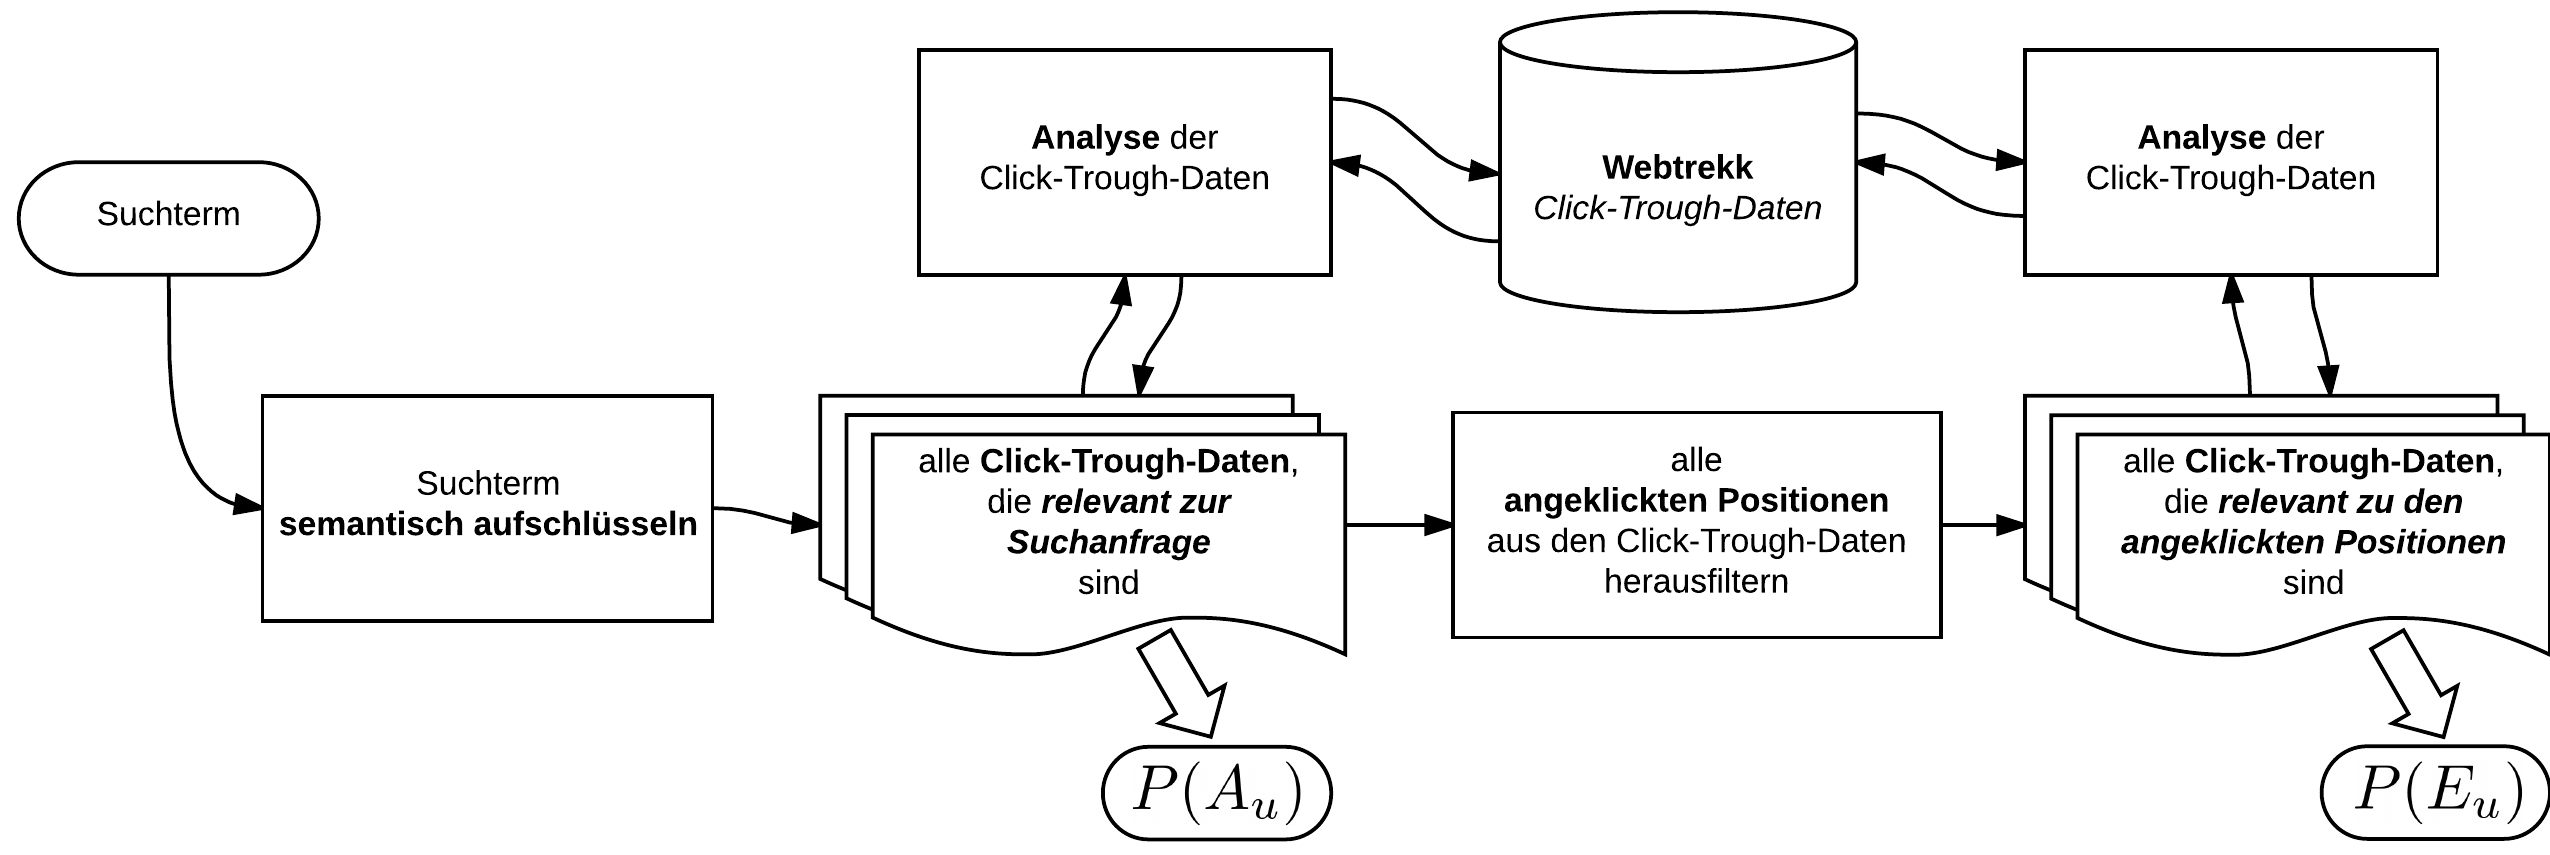
\includegraphics[width=\linewidth]{gfx/WahrscheinlichkeitswerteCTDaten}
\vspace{-2.5em}
\end{figure}

\paragraph{Click-Through-Daten der Dokument-Wahrscheinlichkeit $P(A_{u})$ filtern}
Für die Berechnung der Dokument-Wahrscheinlichkeit verwenden wir das weiter oben in Kapitel \ref{sec:Reranking:Methodik:Click-Through-Daten:Click-Through-DatenAuswertungen} angesprochene Verfahren zur Suchterm-Segmentierung, um \textit{alle für die Suchanfrage relevanten Click-Through-Daten} zu lesen. Aus diesen Click-Through-Daten können wir mithilfe der vorgestellten Formel für $P(A_{u})$ die Wahrscheinlichkeit berechnen, dass ein Dokument aufgrund seines Suchsnippets im Suchergebnis angeschaut wird.  

\paragraph{Click-Through-Daten der Positions-Wahrscheinlichkeit $P(E_{u})$ filtern}
Für die Berechnung der Positions-Wahrscheinlichkeit filtern wir aus den für die Dokument-Wahrscheinlichkeit
gelesenen Click-Through-Daten \textit{alle angeklickten Positionen} heraus. Zu diesen Positionen lesen wir dann unabhängig des Suchterms, alle Click-Through-Daten, in denen auf diese Positionen geklickt wurde. Aus den resultierenden Click-Through-Daten können wir mithilfe der vorgestellten Formel für $P(E_{r_{u}})$ die Wahrscheinlichkeit berechnen, dass ein Dokument aufgrund aufgrund seiner Position im Suchergebnis angeschaut wird.

\subsubsection{Klick-Wahrscheinlichkeit mit PBM berechnen}
\label{sec:Reranking:Methodik:Result-RerankingPBM:Klick-Wahrscheinlichkeit}

Wie in Kapitel \ref{sec:Grundlagen:Grundbegriffe:Result-RerankingPBM:AnsatzSucheEinbinden} angesprochen, werden wir unseren Reranking-Algorithmus in die Aufbereitung der Suchresultate aus der Solr-Suche integrieren. Wir werden die Click-Through-Daten wie im vorherigen Teil der Methodik besprochen aufbereiten. Auf diesen werden wir dann unseren Reranking-Algorithmus anwenden, um die CTRs der einzelnen Dokumente des Suchergebnisses zu berechnen. 

\paragraph{Reranking-Algorithmus kann nur die Top-N-Ergebnisse betrachten}
Wir müssen bei unserem Ansatz beachten, dass die Solr durch die Pagination-Funktion~(siehe \cite{Pagination}) nur die Top-N-Ergebnisse zurückgibt. Dadurch sehen wir nur einen Teil der Suchergebnisse. Um sicherzustellen, dass wir möglichst viele relevante Suchergebnisse berücksichtigen, werden wir die ersten 100 Suchergebnisse der Solr im Reranking-Algorithmus verarbeiten. Aus der daraus resultierenden Liste der Suchergebnisse, filtern wir die ersten 20 Ergebnisse und stellen diese dar. Für die Untersuchung des Reranking-Algorithmus werden wir uns bei der Auswertung jeweils auf die Seite 1 der Suchergebnisse konzentrieren. Bei Springermedizin somit auf die ersten 20 Suchresultate. Die Pagination der Folgeseiten der Suchresultate werden wir nicht untersuchen. Würden wir diesen Algorithmus in einer Live-Applikation\footnote{Mit Live-Applikation wird hier eine öffentliche, für Kunden zugängliches Applikation beschrieben} implementieren wollen, müssten wir uns für die Ausspielung der Folgeseiten des Suchresultats einen zusätzlichen Lösungsansatz überlegen. Mit diesem müsste erreicht werden, dass die Solr die durch den Reranking-Algorithmus bereits ausgespielten Suchresultate, nicht mehrfach ausspielt.

\paragraph{Ausarbeitung des effektiven Algorithmus}
Unseren Reranking-Algorithmus bauen wir auf der in Kapitel \ref{sec:Grundlagen:Grundbegriffe:Result-RerankingPBM:Grundlagen} vorgestellten Formel des PBMs auf. Wie wir in der Analyse der Grundlagen in Kapitel \ref{sec:Grundlagen:Grundbegriffe} festgestellt haben, reicht die triviale Umsetzung unseres Klick-Modells für unseren Algorithmus nicht aus. Wir haben darum verschiedene Lösungsansätze für die Problemstellungen vorgestellt. Mithilfe einiger dieser Lösungsansätzen, wollen wir nun den effektiven Algorithmus ausarbeiten.

\subsubsection{Smoothing-Faktor in PBM einführen}
\label{sec:Reranking:Methodik:Result-RerankingPBM:SmoothingPBM}

Wir wissen dass eine Wahrscheinlichkeit einen Wert zwischen 0 und 1 besitzt. Dadurch können Nullwerte entstehen. Das PBM multipliziert die Positions- und Dokument-Wahrscheinlichkeit miteinander, um die Klick-Wahrscheinlichkeit zu berechnen. Wir müssen aber davon ausgehen, dass es Dokumente im Suchresultat geben kann, deren Position nie angeklickt wurde und umgekehrt. Multiplikationen mit Null ergeben immer einen Nullwert.  Wir führen darum an dieser Stelle einen \textit{Smoothing-Faktor} ein:

\begin{figure}[H]
\centering
\vspace{-1em}
\caption[Berechnung der CTR mittels PBM]{Berechnung der CTR mittels PBM}
\label{fig:BerechnungCTRmittelsPBM}
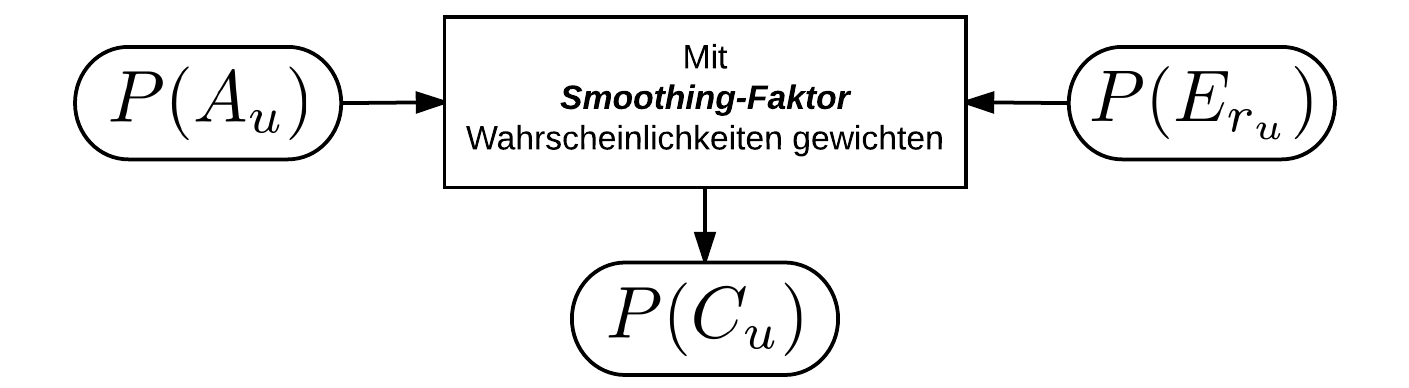
\includegraphics[width=.5\linewidth]{gfx/BerechnungCTRmittelsPBM}
\vspace{-2.5em}
\end{figure}

\paragraph{Mit Smoothing-Faktor Wahrscheinlichkeitswerte gewichten}
Der Smoothing-Faktor soll zwei Probleme lösen. Zum Einen wollen wir einen Wahrscheinlichkeitswert trotz der Multiplikation mit Null beachten (1). Zum Anderen wollen wir die im vorherigen Absatz beschriebene Gewichtung abhängig des Relevanz-Feedbacks, in den Algorithmus einbeziehen (2). Wir transformieren dazu das Produkt der beiden Wahrscheinlichkeiten in eine gewichtete Summe, indem wir eine \textit{Smooting-Konstante} einführen. Die Smoothing-Konstante $\lambda$ soll die Gewichte der beiden Klick-Wahrscheinlichkeiten $P(E_{r_{u}})$ und $P(A_{u})$ zu eins aufsummieren. Wir verwenden dazu das \textit{Exponential Smoothing Modell}~(siehe \cite{ExpSmoothing}). Bilden wir dieses Modell auf den PBM basierten Algorithmus ab, sieht die Formel für die CTR (= $P(C_{u})$) wie folgt aus:
  
\vspace{-1.5em}
\begin{equation}
	P(C_{u}) = \lambda\cdot P(E_{r_{u}}) + (1 - \lambda)\cdot P(A_{u})
\end{equation}
\vspace{-1.5em}

\subsubsection{Smoothing-Faktor abhängig der Position im Suchresultat definieren}
\label{sec:Reranking:Methodik:Result-RerankingPBM:VerhaeltnisKlick-Wahrscheinlichkeiten}

Die in Kapitel \ref{sec:Grundlagen:Grundbegriffe:Result-RerankingPBM:Grundlagen} angesprochene Studie \cite{pbm} hat aufgezeigt, dass das PBM sich stark an der Position eines Dokumentes im Suchresultat orientiert und dies negative Einflüsse auf die Prognose der CTR haben kann. Die Klick-Wahrscheinlichkeit $P(E_{r_{u}})$ darf darum nicht zu viel Einfluss haben. Aus eigener Erfahrung wissen wir zudem, dass die ersten Dokumente im Suchresultat immer zuerst gesehen werden. Die dahinter gelisteten Dokumente werden fortlaufend analysiert. Dies bestätigt die in Abb. \ref{fig:Grundlage:AnalyseKlicksPositionen} dargestellte Analyse der Klicks auf die ersten 20 Positionen eines Suchergebnisses. Wir sollten darum darauf achten, dass je \textit{schlechter} die Position des angeklickten Dokumentes im Suchresultat der Solr ist, desto \textit{höher} das Relevanz-Feedback zu bewerten ist. 
\\
\\
Das machen wir, indem wir für die Berechnung der CTR des Dokumentes, den Smoothing-Faktor abhängig der Position im Suchresultat definieren. Dadurch können wir das Verhältnis zwischen Klick-Wahrscheinlichkeit der Position und Klick-Wahrscheinlichkeit des Dokumentes steuern. Als Grundlage hierbei dient uns die Position des Suchresultats der Solr. Wie die Aufteilung dazu aussehen wird, sehen wir folgend:

\begin{table}[H]
\centering
\vspace{-.75em}
 \caption[Smoothing-Faktor abghängig der Position im Suchergebnis]{Smoothing-Faktor abghängig der Position im Suchergebnis}
\label{tab:VerhaeltnisKlick-WahrscheinlichkeitenPositionDokument}
\vspace{-.5em}
\footnotesize
\renewcommand*{\arraystretch}{1.2}
\begin{tabular}{lcc} \hline
	\textbf{Position} & \textbf{Verhältnis Position zu Dokument} & \textbf{Wert des Smoothing-Faktors $\lambda$}\\ \hline
	1 bis 10 & 1:1 & 0.50\\ \hline
	11 bis 20 & 1:2 & 0.34\\ \hline
	größer 20 &  1:3 & 0.25\\ \hline
 \end{tabular}
\vspace{-2em}
\end{table}

Für die Suchresultate mit einer Position über 20, verstärken wir die Gewichtung der Klick-Wahrscheinlichkeit des Dokumentes erheblich. Wir gehen davon aus, dass bei Klicks auf Dokumente mit einer solch hohen Position, die suchende Person die Suchresultate genau analysierte, bevor sie ein Dokument angeklickt hat.

\subsection{Vergessen der alten Daten}
\label{sec:Reranking:Methodik:Vergessen}

Ein Algorithmus zur Berechnung von Wahrscheinlichkeiten muss sich ein gewisses Grundwissen aneignen. Dies geschieht üblicherweise durch Trainingsdaten. Genauso muss er alte Daten wieder vergessen können, um Overfitting\footnote{Überanpassung des Algorithmus durch zu viele (falsche oder veraltete) Daten} zu vermeiden. 

\subsubsection{Durch Webtrekk ist kein komplexer Lern-Algorithmus notwendig}
\label{sec:Reranking:Methodik:Vergessen:Lern-Algorithmus}

Durch Webtrekk haben wir eine Wissensbasis, die sich stetig und zeitnah aktualisiert. So muss der Algorithmus nicht ständig neues Wissen lernen und altes vergessen, sondern er kann direkt auf diese Wissensbasis zugreifen. Dies geschieht, indem zur Laufzeit\footnote{Unter Laufzeit wird in diesem Fall der Zeitpunkt der direkte Abfrage während der Suchanfrage bezeichnet} Analysen gegen Webtrekk über eine frei definierbare Periode gemacht werden. Dadurch kann \textit{Overfitting} durch veraltete Daten vermieden werden. Deshalb verwenden wir keinen komplexen Lern-Algorithmen wie in \cite{IWUSBI} vorgestellt.

\subsubsection{Die Klick-Wahrscheinlichkeit ist kein absoluter Wert für die Userrelevanz}
\label{sec:Reranking:Methodik:Vergessen:Relevanzfeedback}

Nun könnten wir die Klick-Wahrscheinlichkeit als absoluten Wert für die \textit{Userrelevanz} betrachten. Dies wäre jedoch falsch, wie in Kapitel \ref{sec:Grundlagen:Grundbegriffe:SemantikUserInteraktionen:RankExamination} analysiert, müssen wir davon ausgehen, dass viele User der Qualität der Suchmaschine vertrauen. Diese betrachten die \glqq Top-Suchresultate\grqq{} als die relevanten Suchresultate. Denkbar wäre auch, dass User unabsichtlich das falsche Dokument anklicken und dadurch die CTR eines Dokumentes verfälschen. Dadurch kann ein \textit{Overfitting} des Algorithmus durch nicht relevante Click-Through-Daten entstehen.

\subsubsection{Overfitting vermeiden}
\label{sec:Reranking:Methodik:Vergessen:Overfitting}

Um das angesprochene Overfitting zu vermeiden, darf der Algorithmus nicht immer anschlagen. Wir müssen sicherstellen, dass vereinzelt \textit{zufällige Dokumente} in den \glqq Top-Suchresultaten\grqq{} angezeigt werden. So können auch andere Dokumente in den Fokus des Users gerückt werden. Das System fährt sich dadurch nicht auf falschen Annotationen fest. 

\paragraph{Zusätzliche Varianz durch Zufallsfaktor} 
Mithilfe eines Zufallsfaktors kann eine solche Varianz\footnote{Mit Varianz bezeichnen wir hierbei eine Abweichung vom berechneten Erfahrungswert} in den Klick-Modell basierten Algorithmus gebracht werden. Konkret wollen wir den Reranking-Algorithmus beeinflussen, indem wir mithilfe eines Zufallsfaktors, Abweichungen von der berechneten Klick-Wahrscheinlichkeit eines Dokumentes provozieren. Den dazu verwendeten Zufallswert $X_{u}$,  lassen wir uns als positive ganze Zahl generieren. Er soll eine Zufallsposition im Suchergebnis darstellen:

\vspace{-1.75em}
\begin{equation}	
	X_{u} \in \lbrace \text{Positionen im Suchresultat} \rbrace \subset \mathbb{N}
\end{equation}
\vspace{-1.5em}

\subsubsection{Zufallsfaktor mittels Smoothing-Faktor in 	die Sortierung der Suchergebnisse einbauen}
\label{sec:Reranking:Methodik:Vergessen:ZufallsfaktorSmoothing}

Mit unserem berechneten Zufallswert können wir nun die angesprochenen Abweichungen in die Klick-Wahrscheinlichkeiten der Dokumente einbauen. Wie bereits in Kapitel \ref{sec:Grundlagen:Grundbegriffe:SemantikUserInteraktionen:DocumentAttraction} thematisiert, werden viele Suchresultate nie und deren Position selten bis gar nicht angeklickt. Sie haben darum keine Click-Through-Daten. Deren Klick-Wahrscheinlichkeit ist entweder Null oder sehr klein. Der Zufallswert soll darum nur leichte Einflüsse in die Klick-Wahrscheinlichkeit haben.

\paragraph{Effektive Position im Suchergebnis mittels Smoothing-Faktor berechnen} 
Ein direkter Einbau in die Klick-Wahrscheinlichkeitsberechnung ist jedoch schwierig, da die Wahrscheinlichkeitsverteilungen auf die Dokumente im Suchergebnis stark schwanken und sich der Einfluss des Zufallswertes dadurch stetig verändert. Wir werden darum die Klick-Wahrscheinlichkeit und den Zufallswert der Dokumente separat verarbeiten und zum Schluss die zwei daraus resultierenden Werte eines Dokumentes, mithilfe eines Smoothing-Faktors gewichtet aufsummieren. Diese Summe dient dann als Relevanz-Wert eines Dokumentes. Das Reranking der Dokumente werden wir anhand dieser Relevanz-Werte durchführen. Die Verarbeitung sieht wie folgt aus:

\begin{figure}[H]
\centering
\vspace{-1em}
\caption[Berechnung der effektiven Position im Suchergebnis mittels Smoothing-Faktor]{Berechnung der effektiven Position im Suchergebnis mittels Smoothing-Faktor}
\label{fig:BerechnungRerankedPosition}
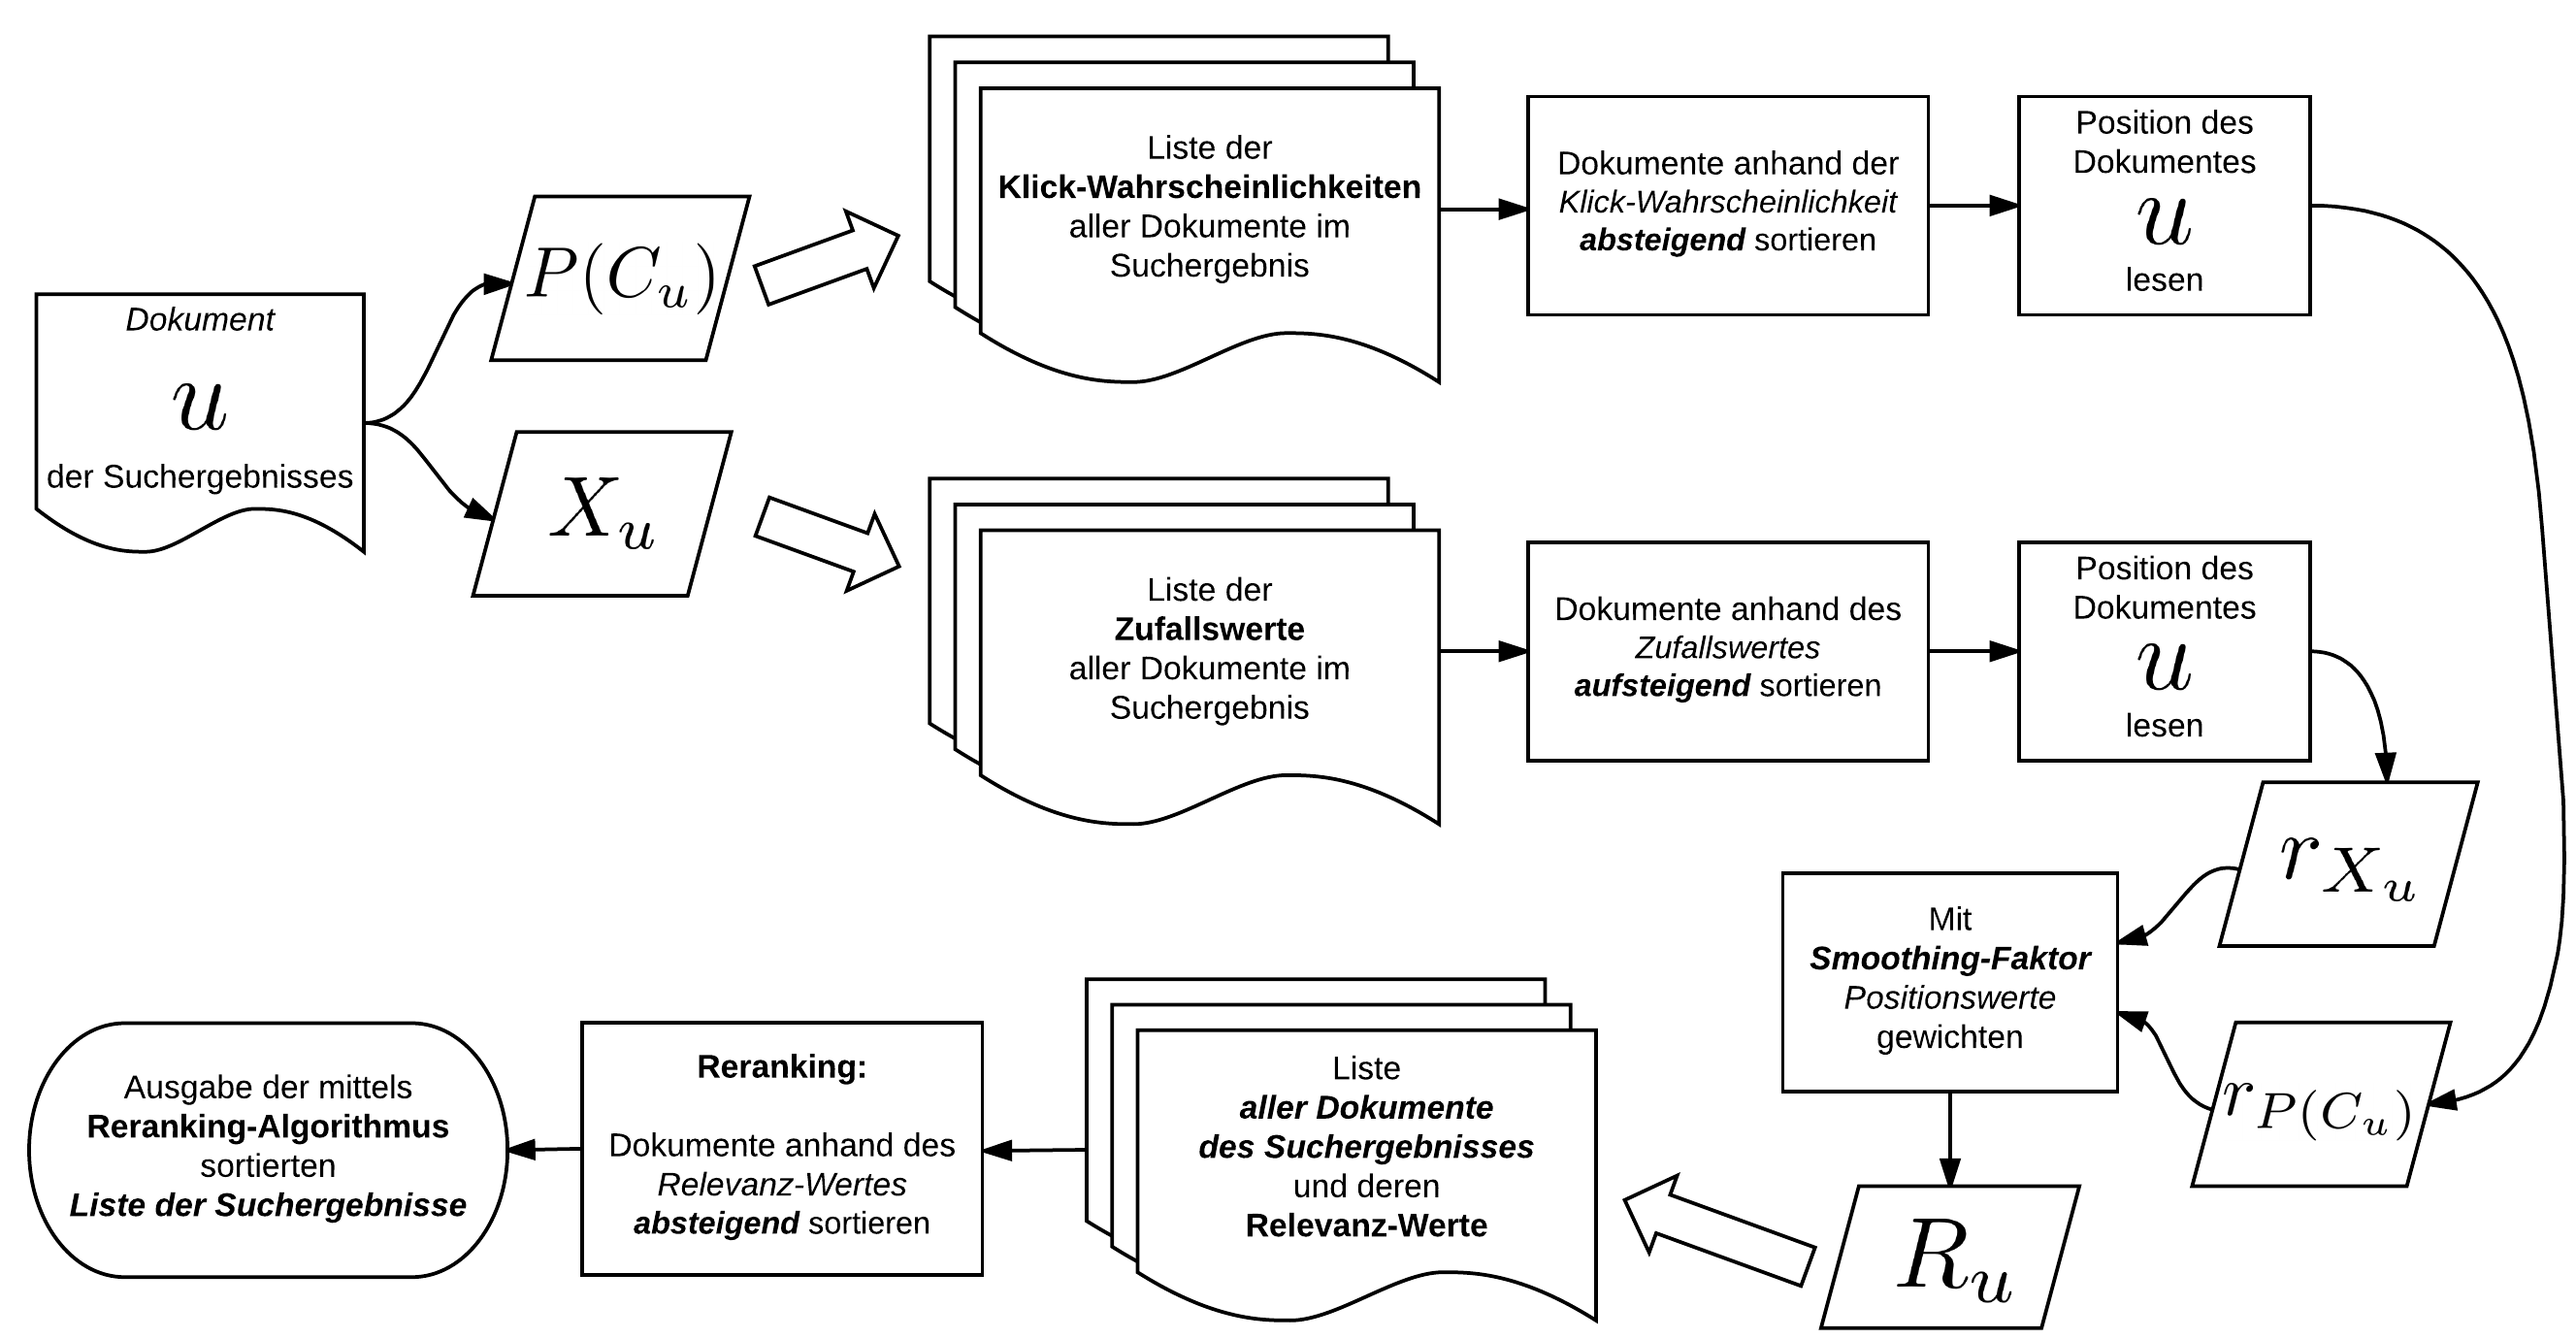
\includegraphics[width=\linewidth]{gfx/BerechnungRerankedPosition}
\vspace{-2.5em}
\end{figure}

Aus den Klick-Wahrscheinlichkeiten und den Zufallswerten der Dokumente des Suchergebnisses erzeugen wir zwei Listen und sortieren diese wie in der Abbildung beschrieben. Aus diesen Listen können wir für jedes Dokument $u$ jeweils eine Position aus der Liste der Klick-Wahrscheinlichkeiten $r_{P(C_{u})}$ und eine Position aus der Liste der Zufallswerte $r_{X_{u}}$ lesen. Aus diesen beiden Positionswerten des Dokumentes berechnen wir den effektiven Relevanz-Wert des Dokumentes $R_{u}$. Dazu verwenden wir wieder das \textit{Exponential Smoothing Modell} für den Smoothing-Faktor und berechnen damit die gewichtete Summe der beiden Positionswerte. Wie bereits weiter oben erwähnt, setzen wir den Smoothing-Faktor so an, dass der Zufallswert nur leichte Einflüsse in den effektiven Relevanz-Wert hat. Wir verwenden dazu einen Smoothing-Faktor zwischen 0.05 und 0.1. Den genauen Einfluss-Wert werden wir in der später folgenden Evaluation evaluieren. Folgend die Formel zur Berechnung des effektiven Relevanz-Wertes eines Dokumentes $R_{u}$:

\vspace{-1em}
\begin{equation}
	R_{u} = \frac{1}{\lambda\cdot r_{X_{u}} + (1 - \lambda)\cdot r_{P(C_{u})}}
\end{equation}
\vspace{-1em}

\pagebreak

\paragraph{Reranking des Suchresultats nach $R_{u}$-Wert der Dokumente}
Mithilfe dieser Berechnung erzeugen wir eine Liste von Tupeln mit zwei Komponenten ($R_{u}$, $u$), bestehend aus dem Relevanz-Wert $R_{u}$ und dem Dokument $u$. Diese Liste sortieren wir nach $R_{u}$ absteigend und erzeugen daraus eine neue Liste der in den Tupeln enthaltenen Dokumente $u$. Diese umsortierte Liste ist das Resultat des Rerankings mittels unserem PBM basierten Algorithmus. Diese präsentieren wir zum Schluss dem User, als Suchresultat zur Suchanfrage. 

%Zusammenfassung
%----------------------------------------------------------------

\section{Zusammenfassung}
\label{sec:Reranking:Zusammenfassung}

\paragraph{Stark modifizierter Reranking-Algorithmus}
Mithilfe des PBM können wir trotz stark begrenzter Click-Trough-Informationen ein relativ gutes Relevanz-Feedback gewinnen, welches wir im Reranking-Algorithmus verwenden können. Das Grundgerüst der ausgearbeiteten Algorithmus basiert immer noch auf dem PBM. Wir mussten jedoch einige Modifikationen vornehmen, um den Algorithmus zu erhalten, mit welchem wir nun im nächsten Kapitel die Implementierung durchführen wollen. Diese Modifikationen sind auf die vielen identifizierten Problemstellungen und den daraus folgenden Einarbeitungen der Lösungsansätze in den Algorithmus zurückzuführen. Einige der Modifikationen sind sicherlich der Implementierung im Springermedizin-Umfeld geschuldet. Wir sollten aber davon ausgehen, dass in jedem anderen realistischen Umfeld, ähnliche Problemstellungen auftreten können. Diese praxisnahe Ausarbeitung des Algorithmus ist daher ein guter Test, um die praktische Einsatzfähigkeit des in diesem Kapitel vorgestellten, theoretischen Ansatz zu evaluieren. 

\paragraph{Mittels Smoothing-Faktor Maximum an Informationen verwerten}
Ein wichtiges Hilfsmittel bei der Einarbeitung der Lösungsansätze in der Algorithmus, war der in diesem Kapitel eingeführte Smoothing-Faktor. Mithilfe des Smoothing-Faktors konnten wir die Nullwert-Problematik der Wahrscheinlichkeitsberechnung lösen und die Einflüsse der verschiedenen Faktoren in den Algorithmus besser kontrollieren. Dadurch konnten wir das Maximum an Informationen aus unserem PBM basierten Algorithmus herausholen. 
\\
\\
In der Implementierung und der anschließenden Evaluation wird sich nun zeigen, ob der Lösungsansatz wie angedacht, umgesetzt werden kann und die angestrebten Verbesserungen des Qualitätsmaßes der Suche, erreicht werden können.
